\documentclass[master=elt,masteroption=eg]{kulemt}
\setup{title={Ontwerp van een RRAM geheugen},
  author={Wouter Diels\and Alexander Standaert},
  promotor={Prof.\,dr.\,ir.\ W. Dehaene},
  assessor={Prof.\,dr.\,ir.\,R. Lauwereins\and Prof.\,dr.\,ir.\, M. Verhelst},
  assistant={B.~Buran \and dr.\,ir.\ S.~Cosemans}}
% De volgende \setup mag verwijderd worden als geen fiche gewenst is.
\setup{filingcard,
  translatedtitle={The best master thesis ever},
  udc=621.3,
  shortabstract={Hier komt een heel bondig abstract van hooguit 500
    woorden. \LaTeX\ commando's mogen hier gebruikt worden. Blanco lijnen
    (of het commando \texttt{\string\pa r}) zijn wel niet toegelaten!
    \endgraf \lipsum[2]}}
% Verwijder de "%" op de volgende lijn als je de kaft wil afdrukken
%\setup{coverpageonly}
% Verwijder de "%" op de volgende lijn als je enkel de eerste pagina's wil
% afdrukken en de rest bv. via Word aanmaken.
%\setup{frontpagesonly}

% Kies de fonts voor de gewone tekst, bv. Latin Modern
\setup{font=lm}
\setup{inputenc=utf8}
% Hier kun je dan nog andere pakketten laden of eigen definities voorzien

% Tenslotte wordt hyperref gebruikt voor pdf bestanden.
% Dit mag verwijderd worden voor de af te drukken versie.
\usepackage[pdfusetitle,colorlinks,plainpages=false]{hyperref}

%%%%%%%
% Om wat tekst te genereren wordt hier het lipsum pakket gebruikt.
% Bij een echte masterproef heb je dit natuurlijk nooit nodig!
\IfFileExists{lipsum.sty}%
 {\usepackage{lipsum}\setlipsumdefault{11-13}}%
 {\newcommand{\lipsum}[1][11-13]{\par Hier komt wat tekst: lipsum ##1.\par}}
%%%%%%%

%\includeonly{hfdst-n}
\begin{document}

\begin{preface}
  Dit is mijn dankwoord om iedereen te danken die mij bezig gehouden heeft.
  Hierbij dank ik mijn promotor, mijn begeleider en de voltallige jury.
  Ook mijn familie heeft mij erg gesteund natuurlijk.
\end{preface}

\tableofcontents*

\begin{abstract}
  In dit \texttt{abstract} environment wordt een al dan niet uitgebreide
  samenvatting van het werk gegeven. De bedoeling is wel dat dit tot
  1~bladzijde beperkt blijft.

  \lipsum[1]
\end{abstract}

% Een lijst van figuren en tabellen is optioneel
%\listoffigures
%\listoftables
% Bij een beperkt aantal figuren en tabellen gebruik je liever het volgende:
\listoffiguresandtables
% De lijst van symbolen is eveneens optioneel.
% Deze lijst moet wel manueel aangemaakt worden, bv. als volgt:
\chapter{Lijst van afkortingen en symbolen}
\section*{Afkortingen}
\begin{flushleft}
  \renewcommand{\arraystretch}{1.1}
  \begin{tabularx}{\textwidth}{@{}p{12mm}X@{}}
    LoG   & Laplacian-of-Gaussian \\
    MSE   & Mean Square error \\
    PSNR  & Peak Signal-to-Noise ratio \\
  \end{tabularx}
\end{flushleft}
\section*{Symbolen}
\begin{flushleft}
  \renewcommand{\arraystretch}{1.1}
  \begin{tabularx}{\textwidth}{@{}p{12mm}X@{}}
    42    & ``The Answer to the Ultimate Question of Life, the Universe,
            and Everything'' volgens de \cite{h2g2} \\
    $c$   & Lichtsnelheid \\
    $E$   & Energie \\
    $m$   & Massa \\
    $\pi$ & Het getal pi \\
  \end{tabularx}
\end{flushleft}

% Nu begint de eigenlijke tekst
\mainmatter

\chapter{Inleiding}
\label{inleiding}

Vandaag de dag is elektronica niet meer uit het leven weg te denken. Van de smartphone tot het digitaal horloge, van de boordcomputer in de moderne wagen tot de microprocessor in de vaatwasser, overal vind je wel elektronica terug.
Sinds Gordon Moore ongeveer 50 jaar geleden de uitspraak deed dat het aantal transistoren op eenzelfde oppervlakte per twee jaar zou verdubbelen \cite{Moo65}, is de industrie er over het algemeen goed in geslaagd dit te verwezenlijken. Dit leidde tot de snelle en uiterst complexe chips die we vandaag allemaal goedkoop aankopen.

Naarmate de processorkracht groter werd, steeg ook de vraag voor grotere en snellere geheugens om deze processorkracht ook effectief uit te buiten. Static Random Access Memory (SRAM) blijft een populaire keuze voor snelle ingebedde geheugens, maar heeft het nadeel vluchtig te zijn: eenmaal de voedingspanning wordt afgeschakeld, verdwijnt de informatie. Flash-geheugens, door veel mensen gebruikt voor massa-opslag in USB-sticks of SSDs, hebben ook hun weg gevonden tot het ingebedde domein en behoren wel tot de klasse van niet-vluchtige geheugens.
Het blijkt echter bijzonder moeilijk om flash-geheugens verder te verkleinen \cite{Pra10}.

Onderzoek naar nieuwe geheugens is dan ook onontbeerlijk. Zo zijn er al nieuwe nieuwe kandidaten in opmars die hoopgevende tekens geven om te concurreren met (ingebedde) flash-geheugens. MRAMs (Magnetic RAMs) en in het bijzonder STT-RAM (Spin-Transfer Torque) zullen op termijn een belangrijke rol gaan spelen.

Een andere kandidaat is Resistive RAM (RRAM of ReRAM). Daar waar SRAM- en flash-cellen de informatie bevatten via het al dan niet aanwezig zijn van lading, bevat een RRAM-cel informatie door een bepaalde elektrische weerstand aan te nemen. RRAM zou geen problemen hebben om nog even op de klassieke manier mee te schalen en is dus zonder meer een interessante piste om te onderzoeken. Bovendien zou het gefabriceerd kunnen worden met goedkopere processen dan flash-geheugens - bij flash-geheugenfabricatie zijn vaak dure extra maskers vereist.

\section{Doel en afbakening van dit werk}
Dit werk beschrijft het ontwerp van een 4MByte RRAM-geheugen voor ingebedde toepassingen. De doelstelling is een pareto-optimaal (dynamische energie-snelheid-oppervlakte) werkend circuit te ontwerpen, gewapend tegen variabiliteit - ongecorreleerde gedragsvariaties van componenten. Het ontwerp houdt rekening met data-retentie bij het uitlezen van bits. De analyse focust op de leesbewerking, de schrijfbewerking valt buiten het bereik van dit werk. [Er worden wel mogelijke oplossingen aangereikt, maar deze werden niet uitdrukkelijk onderzocht]

Voor de leesbewerking wordt het geheugen-element gemodeleerd als een weerstand waarvan de nominale weerstandswaarde afhangt van de celtoestand. Wanneer variabiliteit wordt onderzocht, zal deze weerstandswaarde een stochastische variabele worden met een normale verdeling.

Temperatuursvariaties werden niet in rekening genomen, maar aangezien dit een globale variabele is en het systeem differentieel werkt, wordt niet verwacht dat de performantie aanzienlijk zal verminderen.

Alle data die worden getoond, komen voort uit Spectre-simulaties met 45nm PTM transistormodellen.

\section{Structuur van de tekst}
In hoofdstuk \ref{cell} zal de technologie van een RRAM geheugen uiteengezet worden, alsook diens toepassingen. Ook zal het elementaire principe om uit een weerstand een nuttig elektrisch signaal te vormen uitgelegd worden. In hoofdstuk \ref{architecture} wordt het geheugensysteem vanuit vogelperspectief besproken. Er wordt hier ook aangehaald wat de tunebare parameters zijn van de architectuur. Voor een robuuste, snelle en laag-energetische leesoperatie uit te voeren is het belangrijk het geheugenelement te combineren met een zorgvuldig gekozen impedantie, dit wordt onderzocht in hoofdstuk \ref{loadanalysis}. Uiteindelijk zal er een bitstream moeten gegenereerd worden aan de uitgang van het systeem, de sense amplifier zorgt hiervoor en wordt besproken in hoofdstuk \ref{sensamp}.
In de geheugenstructuur zijn ook bepaalde logische (digitale) operaties nodig om op basis van het opgegeven adres de juiste cel aan te spreken, de hiervoor gebruikte blokken worden beschreven en geanalyseerd in hoofdstuk \ref{periphery}.
Ten slotte zal in hoofdstuk \ref{timing-optimization} de timing van controlesignalen onderzocht worden en hoe het systeem te optimaliseren door middel van de architectuurparameters te tunen.
\chapter{Geheugencel}
\label{cell}
Elk geheugen bestaat uit een verzameling individuele cellen die op een of andere manier informatie bevatten.
In dit hoofdstuk wordt eerst dieper ingegaan op de manier waarom een R-RAM geheugencel informatie bevat en vervolgens hoe deze informatie [elektrisch] kan worden uitgelezen.

\section{Memristor}
Het essentiële element van een R-RAM geheugencel is ontegenspreekbaar de zogenaamde memristor.
De memristor wordt ook wel gezien als de 4\textsuperscript{e} passieve component, naast de weerstand, spoel en condensator.

\subsection{Theoretisch principe}
In 1971 publiceerde Leon Chua een artikel waarin hij opmerkte dat er voor de 4 fundamentele circuitvariabelen (de spanning v, stroom i, lading q en fluxbinding $\lambda$\footnote{$\lambda(t) =  \int^{t}_{-\infty} v(\tau) \, d\tau $, voor een ideale inductantie is dit hetzelfde als magnetische flux: $\lambda = \phi$ }) van 6 mogelijke onderlinge relaties er slechts 5 gekend waren: $q(t) =  \int^{t}_{-\infty} i(\tau) \, d\tau $, $\lambda(t) =  \int^{t}_{-\infty} v(\tau) \, d\tau $, $v(t)=R*i(t)$, $q(t)=C*v(t)$ en $\lambda(t) = L*i(t)$ volgen uit de wetten van Maxwell en uit de definities van de weerstand, spoel en condensator, maar er ontbrak een relatie tussen $\lambda$ en q.\cite{Chu71} Hij suggereerde dat er een 4e nog niet ontdekte passieve 2-pool moest bestaan die dit verband herbergde.
Uit zijn wiskundige berekeningen kwam hij tot de conclusie dat deze component zich ogenblikkelijk als een weerstand zou gedragen, maar dat de weerstandswaarde verandert aan de hand van het verloop van de stroom in de tijd. Gebaseerd op deze conclusie doopte hij deze component de memristor (een contractie van memory en resistor).

\subsection{Fysische werking}
Chua beëindigde zijn artikel met te erkennen dat er op dat moment nog geen fysische memristor was ontdekt, maar dat dit in de toekomst wel kon gebeuren, al dan niet zelfs per ongeluk. Hij gaf zelfs aan dat er misschien al in die tijd materialen met memristorkarakteristieken gebruikt werden, maar dat men hier over keek. Hij zou gelijk krijgen.


\subsection{Toepassingen}


\section{Memristor in een geheugenstructuur}

In dit werk wordt gebruik gemaakt van een \emph{1 Transistor, 1 Resistor} (maar eigenlijk dus een memristor) architectuur, de combinatie van deze twee vormt de geheugencel, maar er zijn nog een paar andere configuraties die zouden toegepast kunnen worden.

\subsection{1T1R}

\subsection{1R}

\subsection{1T1D}



\section{Besluit}


\chapter{Geheugenarchitectuur}
\label{architecture}
De afzonderlijke geheugencellen zullen samengebracht worden in een geheel.
Dit hoofdstuk bespreekt de algemene structuur alsook de vrijheidsgraden die in hoofdstuk \ref{timing-optimization} onderzocht worden om tot een optimaal werkend systeem te komen. Ten slotte zullen ook nog de bouwblokken aangekaart worden die meer uitvoerig besproken worden in de volgende hoofdstukken. 


\section{Cel}
Zoals besproken in hoofdstuk \ref{cell} is dit het bouwblok dat het vaakst terug te vinden is in het geheugensysteem.
De cel bestaat uit een memristor en een transistor (1T1R-cel). De geheugencel heeft drie terminals: de gate van de transistor, die verbonden wordt met een wordline, de source van de transistor, die verbonden wordt met een sourceline en tenslotte de terminal van de memristor, die verbonden wordt met een bitline.
%Een cel waarvan memristor zich in een willekeurige resistieve staat bevindt is een datacel, terwijl de memristor van referentiecellen in een voorgeprogrammeerde en dus gekende resistieve staat verkeert.

\section{Branch}
In een branch worden er een bepaald aantal datacellen verbonden aan één BL en één SL. Dit aantal wordt \emph{Number of Word Lines per Branch} (NoWLpB) genoemd en is een van de vrijheidsgraden van de geheugenarchitectuur. Naast alle datacellen is er ook nog één referentiecel - dit zijn cellen waarvan de resistieve staat voorgeschreven is - verbonden aan de BL en SL van de branch.
Elke BL wordt via een pMOS-transistor (al dan niet met nog een impedantie tussenin) gekoppeld aan de voedingspanning Vdd en via een nMOS-transistor aan de grondspanning Vss. In dit werk is er enkel een nMOS-transistor die de SL verbindt met Vss.\footnote{In een volledig geheugensysteem zou de SL via een pMOS ook nog verbonden zijn met een niet onderzochte spanningsknoop Vdd\_write. De pMOS zou dan worden aangezet voor schrijfwerking.} De nMOS-transistoren aan BL en SL fungeren als schakelaars, de pMOS-transistor wordt daarenboven ook gebruikt als impedantie voor een resistieve spanningsdeling (zie hoofdstuk \ref{loadanalysis}).
Ter illustratie wordt de samenhang tussen cel en branch getoond in figuur \ref{fig:cellbranch}.

\begin{figure}
  \centering
  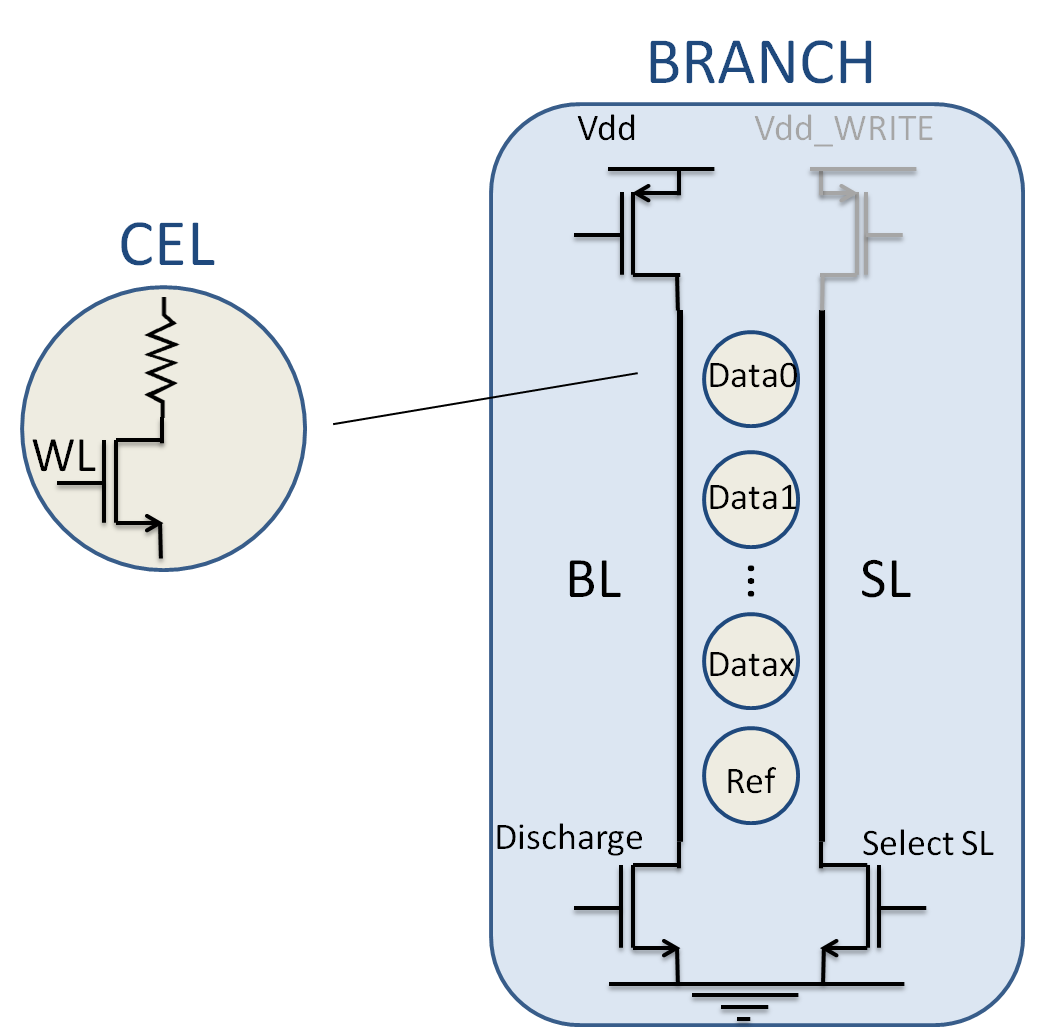
\includegraphics[scale=0.3]{../fig/hfdstk-architecture-cell-branch.png}
  \caption{Een geheugencel en een branch}
  \label{fig:cellbranch}
\end{figure}

\section{Local Block}
Verschillende BLs en SLs worden samengebracht in een local block, waarvan de vrijheidsgraad \emph{Number of BitLines per Local Block} (NoBLpLB) heet. In een LB bevinden er zich dus NoBLpLB x NoWLpB datacellen en NoBLpLB referentiecellen. Ook bevat een local block zowel BL- als WL-decoders. De afzonderlijke BLs worden via passgates verbonden tot een uitgangsknooppunt.
De structuur van een local block is geïllustreerd op figuur \ref{fig:LB}.
De uitgangen van de WL-decoder sturen de data-WLs aan [eventueel met een buffer], de uitgangen van de BL-decoder activeren een spanningsdeling op de BLs.\footnote{Indien schrijfwerking zou toegevoegd worden, zouden de uitgangen van de BL-decoder aan twee AND-poorten worden verbonden; bij leesoperatie brengt de uitgang van de ene AND-poort de resistieve deling op de BL teweeg, bij schrijfoperatie zet de uitgang van de andere AND-poort een pull-up-operatie van de BL naar Vdd\_write op.} De referentie-WL is via een extern signaal verbonden. Voor een gedetailleerdere beschrijving over hoe de decoderuitgangen gebruikt worden, zie sectie \ref{timing}.
Aangezien een LB zowel data- als referentiecellen bevat, gaat een LB twee werkingsmodes hebben: een mode waarbij er één datacel wordt aangesproken en een mode waarbij er een bepaald aantal referentiecellen in parallel wordt aangesproken.
Figuur \ref{fig:LB-details} geeft een meer gedetailleerd beeld van een LB, decoders weggelaten.

\begin{figure}
  \centering
  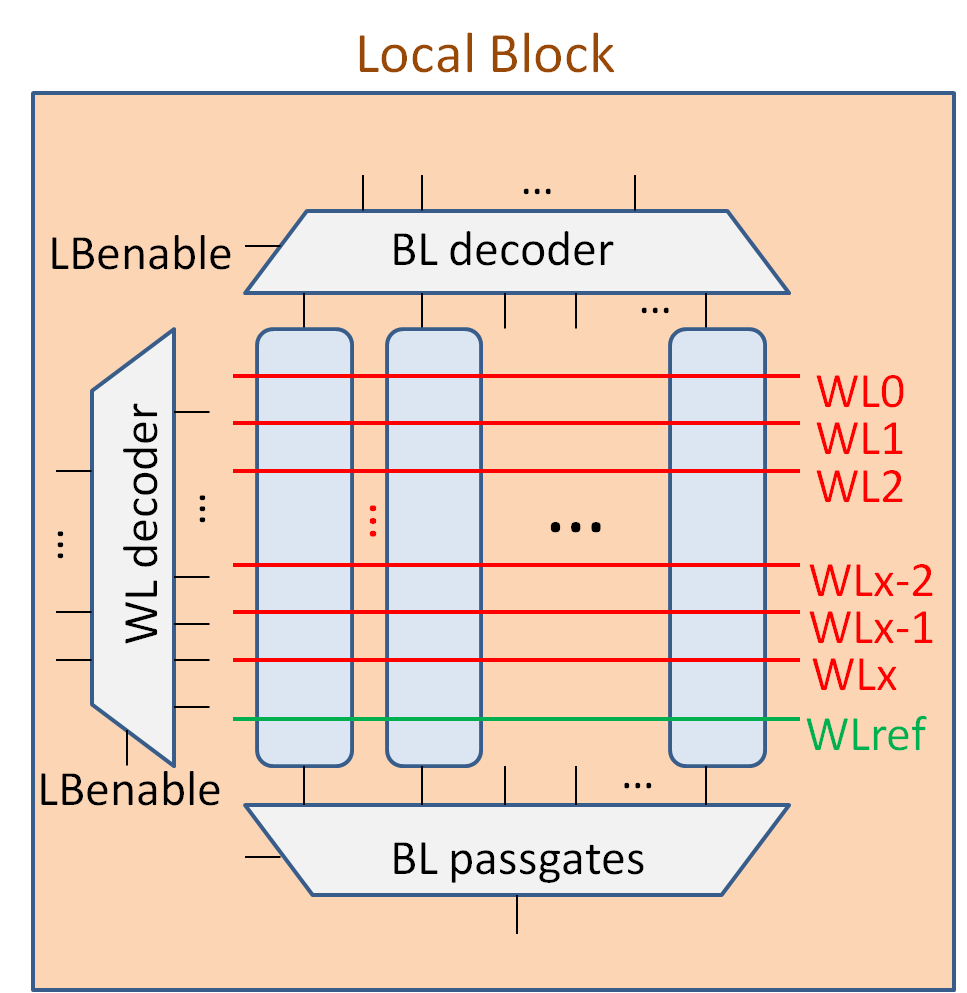
\includegraphics[scale=0.3]{../fig/hfdstk-architecture-localblock.png}
  \caption{Een Local Block}
  \label{fig:LB}
\end{figure}

\begin{figure}
  \centering
  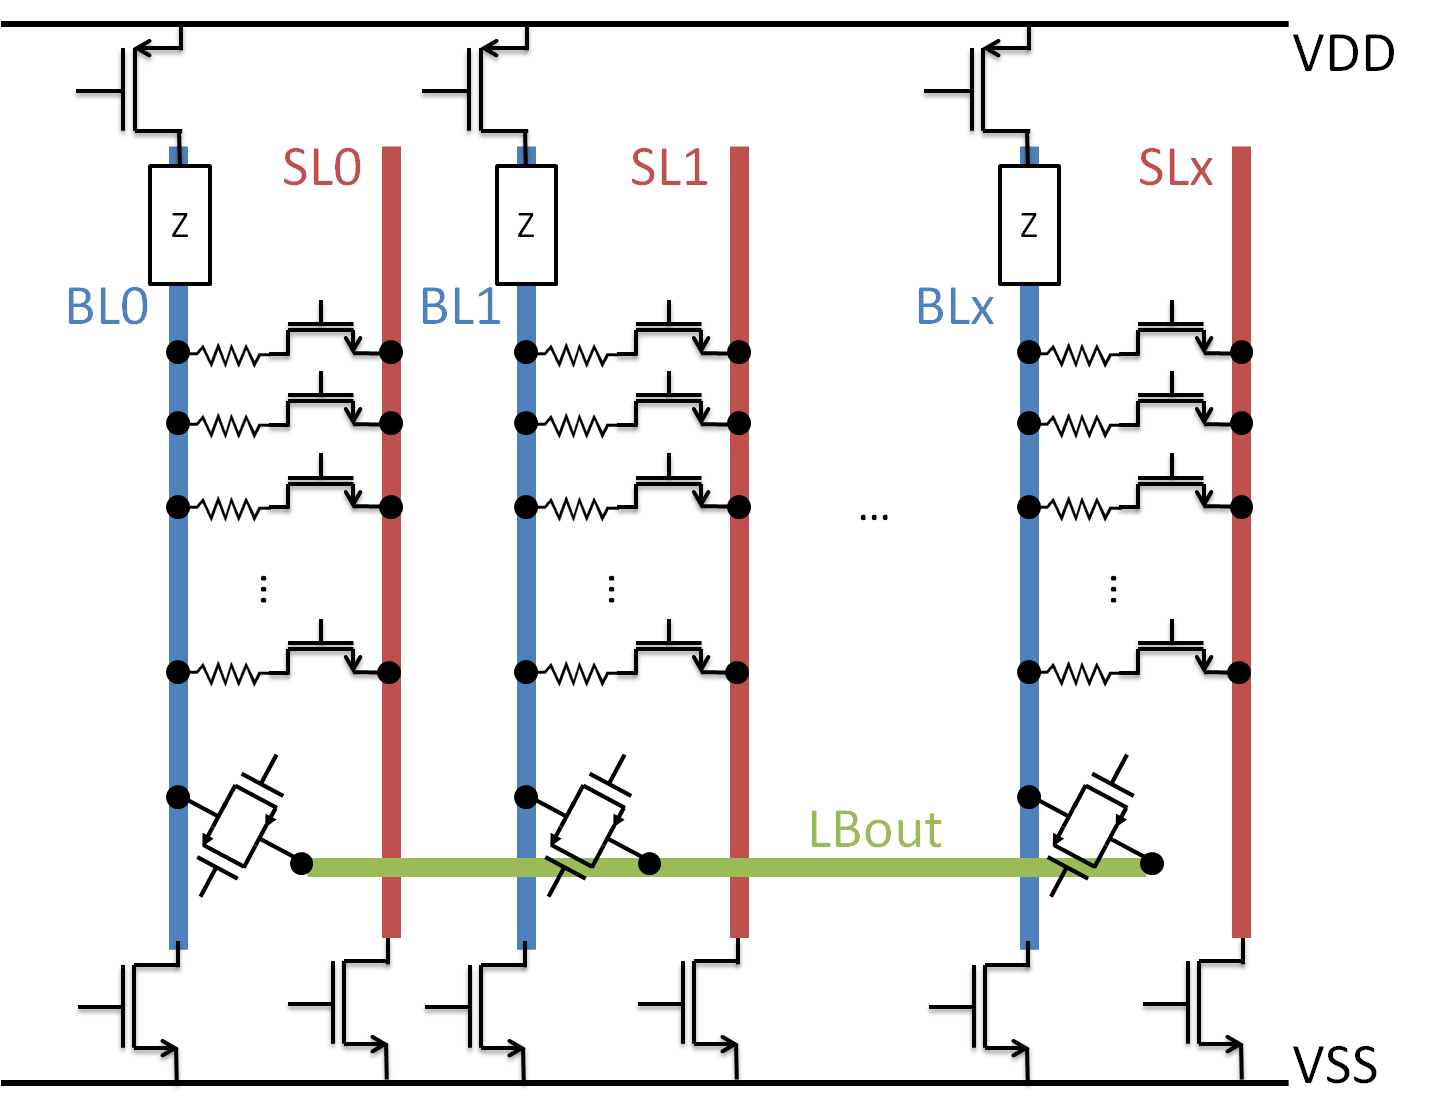
\includegraphics[scale=0.3]{../fig/hfdstk-architecture-LB-details.png}
  \caption{Een meer gedetailleerde illustratie van een LB, decoders zijn weggelaten}
  \label{fig:LB-details}
\end{figure}

\subsection{Datasignaal uitlezen}
Het datasignaal is de spanning op de BL nadat er een resistieve deling is gebeurd, waarbij er stroom vloeit door één cel. De last die hangt aan de voedingsspanning, op figuur \ref{fig:dataread} voorgesteld als een pMOS-transistor, wordt aangeschakeld, alsook de nMOS-transistoren in de cel en aan de sourceline. Er vloeit een stroom langs dit pad: I=Vdd/Rtot, en de spanning op de BL is V=IReq. Om dit datasignaal op de uitgangsknoop van het LB te krijgen, wordt de bijhorende passgate van de BL in kwestie geactiveerd.

\begin{figure}
  \centering
  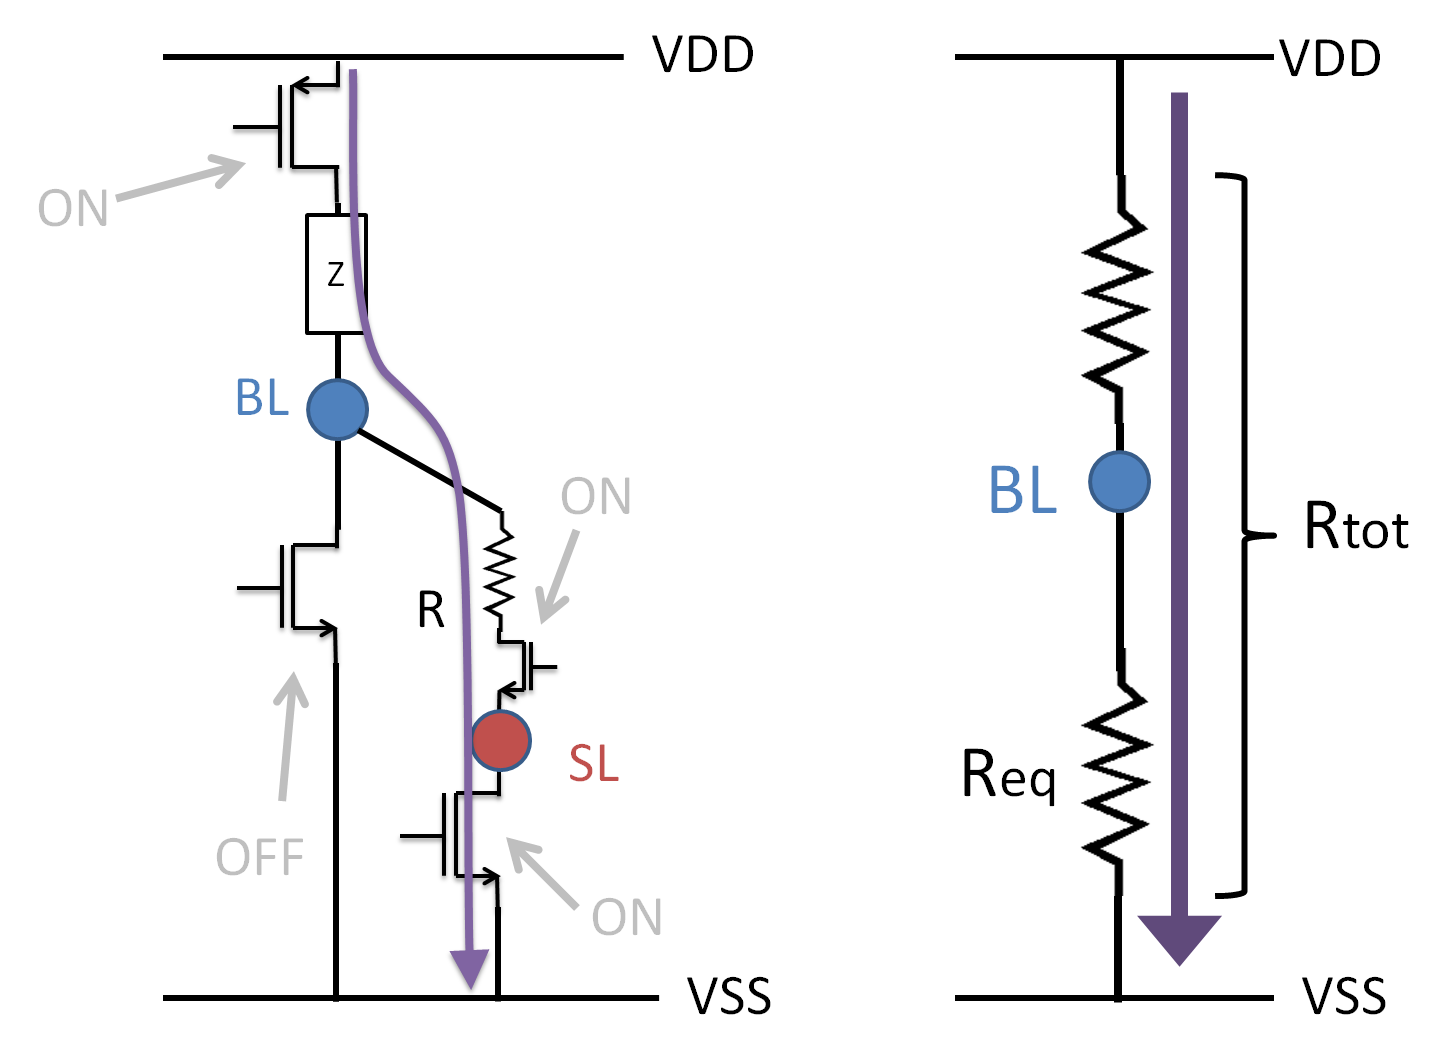
\includegraphics[scale=0.3]{../fig/hfdstk-architecture-datasignal.png}
  \caption{Methodologie om datasignaal te verkrijgen op een BL}
  \label{fig:dataread}
\end{figure}

\subsection{Referentiesignaal uitlezen}
Het referentiesignaal is een spanning die tussen de spanning van een lage resistieve datacel en een hoge resistieve datacel moet liggen. Een dergelijk signaal kan verkregen worden door twee BLs kort te sluiten zoals op figuur \ref{fig:2cellref}. In dit ontwerp zal de kortsluiting gerealiseerd worden door de passgates van de BLs aan te zetten, zo komt het referentiesignaal bovendien ook op de uitgangsknoop te staan. In theorie is het voldoende om 2 BLs [de ene met een HRS cel en de andere met een LRS cel] kort te sluiten om het referentiesignaal te verkrijgen. Er zit echter op de resistieve geheugenelementen variabiliteit: er wordt aangenomen dat $R_{H}$ normaal verdeeld is met $\mu = 32500\Omega$ en $\sigma = 833\Omega$. $R_{L}$ is ook normaal verdeeld met $\mu = 7500\Omega$ en $\sigma = 833\Omega$. Dit betekent dat ook de data-signalen en referentie-signalen stochastische variabelen zijn.
Door echter steeds meer referentiebitlijnen kort te sluiten gaat de spreiding van het referentiesignaal dalen [maar gaat het energieverbruik stijgen]. Bovendien kan men de verwachtingswaarde verschuiven door meer HRS (LRS) referentiegeheugenelementen te gebruiken dan LRS (HRS).

\begin{figure}
  \centering
  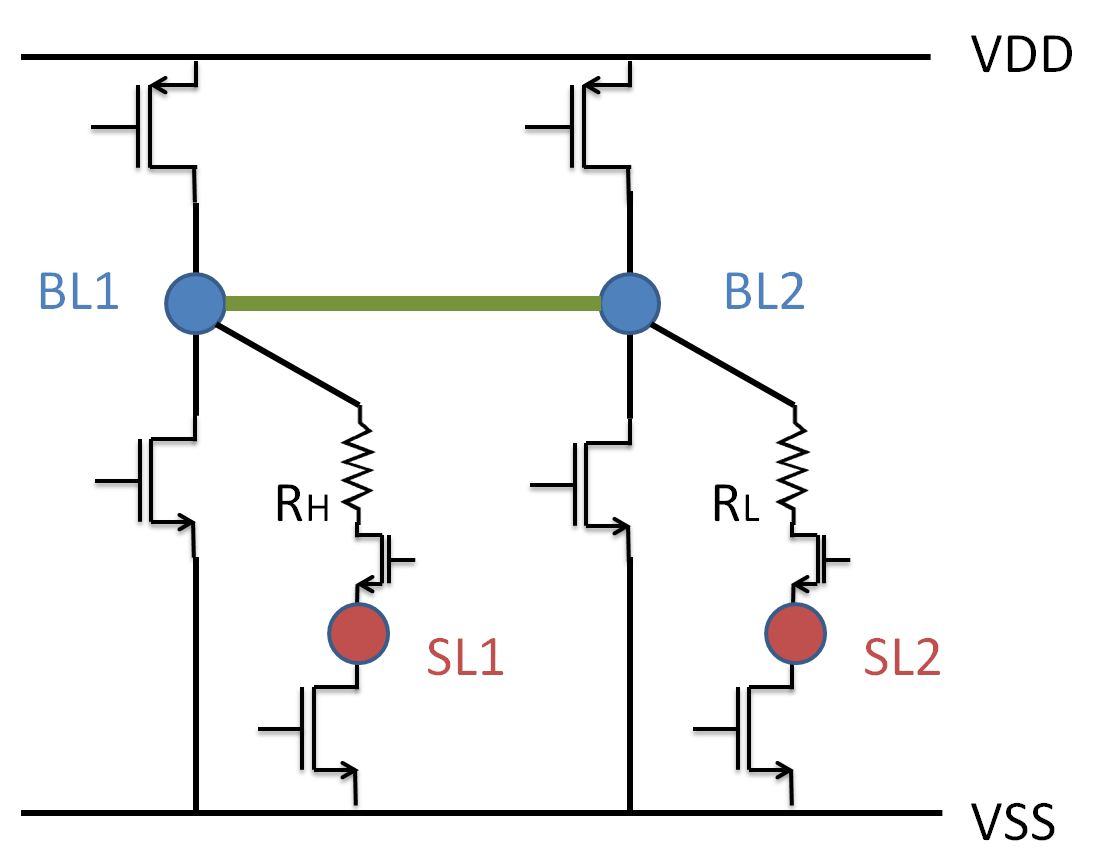
\includegraphics[scale=0.3]{../fig/hfdstk-architecture-ref2cell.png}
  \caption{Topologie om referentiesignaal te verkrijgen}
  \label{fig:2cellref}
\end{figure}

\section{Global Block}
\label{globalblock}
Een global block bestaat uit twee LBs en een sense amplifier (SA) met bijhorende sample-and-hold-schakelaars (S\&H). In het ene LB gaat er een datasignaal geproduceerd worden, in het andere een referentiesignaal (zie figuur \ref{fig:GB}. Vervolgens gaat de SA dit kleine signaalverschil versterken tot een zuivere rail-to-rail output.
Aan de uitgang van het GB verschijnen dan ook de opgevraagde bits.
De laatste architectuurvrijheidsgraad is de \emph{Number of Global Blocks} (NoGB), het totale geheugen bevat dus NoGB x 2 x NoBLpLB x NoWLpB datageheugencellen.

\begin{figure}
  \centering
  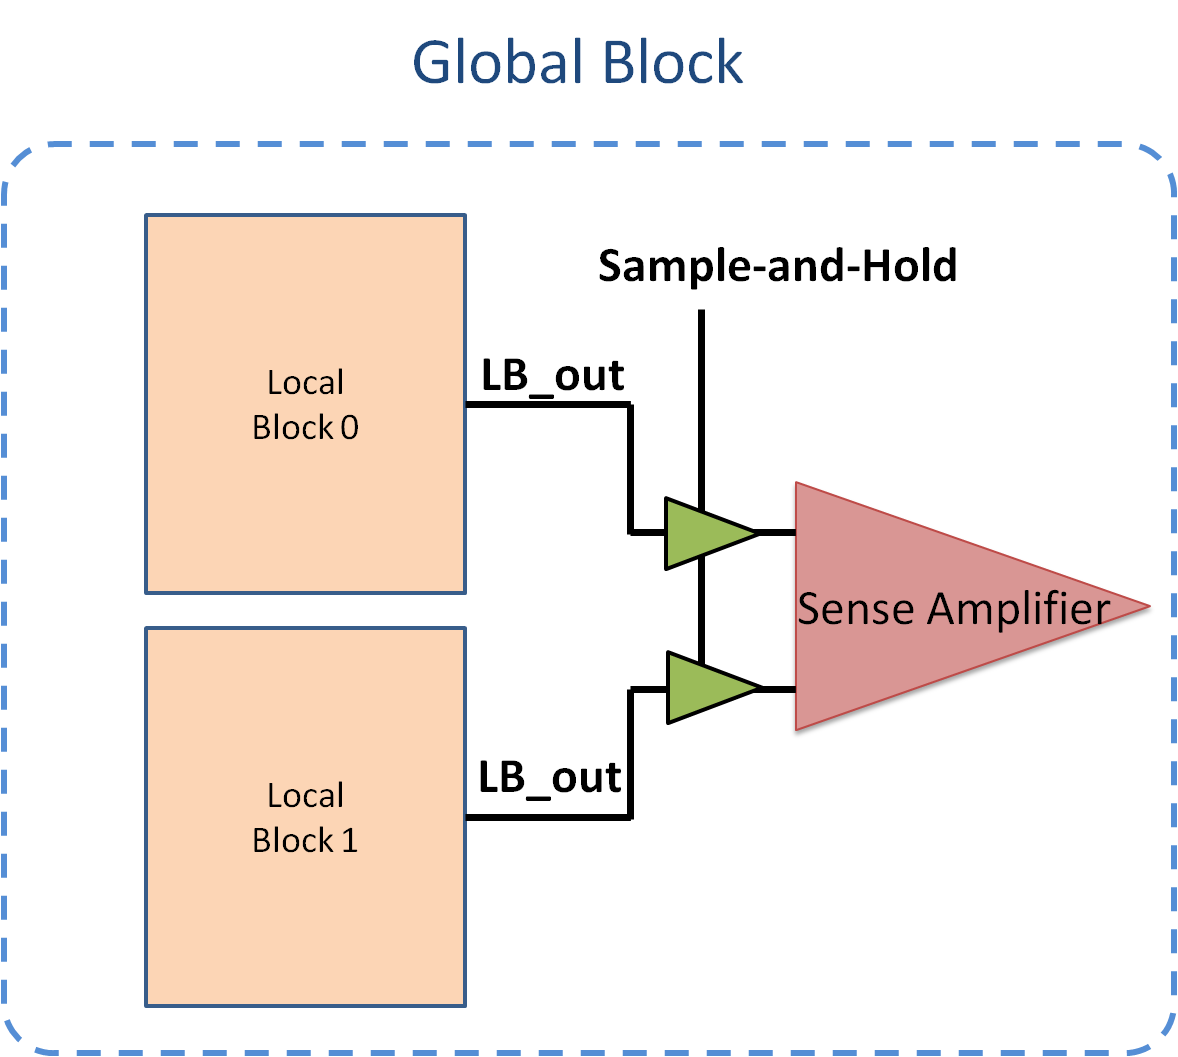
\includegraphics[scale=0.3]{../fig/hfdstk-architecture-globalblock.png}
  \caption{Een Global Block}
  \label{fig:GB}
\end{figure}

\section{Besluit}
De geheugenarchitectuur werd in vogelvlucht overlopen. De kleinste bouwblok is de cel, deze wordt geplaatst in een branch. Verschillende branches vormen samen een local block, dat ook decoders en multiplexers bevat. Twee local blocks en een sense amplifier met bijhorende passgates worden gegroepeerd tot een global block. Het totale geheugen bestaat tenslotte uit een verzameling global blocks.


% ... en zo verder tot
\chapter{Het laatste hoofdstuk}
\label{hoofdstuk:n}
Een hoofdstuk behandelt een samenhangend geheel dat min of meer op zichzelf
staat. Het is dan ook logisch dat het begint met een inleiding, namelijk
het gedeelte van de tekst dat je nu aan het lezen bent.

\section{Eerste onderwerp in dit hoofdstuk}
De inleidende informatie van dit onderwerp.

\subsection{Een item}
De bijbehorende tekst. Denk eraan om de paragrafen lang genoeg te maken en
de zinnen niet te lang.

Een paragraaf omvat een gedachtengang en bevat dus steeds een paar zinnen.
Een paragraaf die maar \'e\'en lijn lang is, is dus uit den boze.

\section{Tweede onderwerp in dit hoofdstuk}
Er zijn in een hoofdstuk verschillende onderwerpen. We zullen nu
veronderstellen dat dit het laatste onderwerp is.

\section{Besluit van dit hoofdstuk}
Als je in dit hoofdstuk tot belangrijke resultaten of besluiten gekomen
bent, dan is het ook logisch om het hoofdstuk af te ronden met een
overzicht ervan. Voor hoofdstukken zoals de inleiding en het
literatuuroverzicht is dit niet strikt nodig.

%%% Local Variables: 
%%% mode: latex
%%% TeX-master: "masterproef"
%%% End: 

\chapter{Besluit}
\label{besluit}
In dit werk werd een RRAM leescircuit ontworpen. De 1T1R-cel die de informatie bevat bestaat uit een minimale transistor en een resistief geheugenelement, de memristor (hoofdstuk \ref{cell}). Voor simulaties werden de geheugenelementen voorgesteld als weerstanden waarvan de impedantie gebaseerd is op hafniumoxidememristoren. Meerdere cellen worden in geheugenmatrices gegroepeerd (hoofstuk \ref{architecture}), aan deze matrices worden decoders en passgates toegevoegd die samen een local block vormen. Een local block kan aan diens uitgang zowel een datasignaal leveren als een referentiesignaal. De uitgangen van 2 LBs worden aan de ingangs-uitgangsknopen van een sense amplifier gehangen; de combinatie van twee LBs en SA heet global block. Data- en referentiesignalen worden opgewekt door een spanningsdeling met een bepaalde lastimpedantie en celimpedantie. Voor het datasignaal vindt er een spanningsdeling plaats op één BL, deze BL-spanning wordt naar de uitgang van het LB overgebracht door de bijhorende passgate te activeren. Voor het referentiesignaal worden er op meerdere BLs spanningsdelingen uitgevoerd, de referentiespanning wordt gevormd door de BLs kort te sluiten aan de uitgang met de passgates. Door meerdere referentiecellen te gebruiken kan de distributie van het referentiesignaal gemanipuleerd worden. Voor een zo groot mogelijk verschil tussen data- en referentiespanning blijkt er een optimale lastimpedantie (hoofdstuk \ref{loadanalysis}). Verschillende topologieën impedantie zijn onderzocht naar BL-spanningsverschil, snelheid en spanningsval over geheugenelement, alsook de invloed van variabiliteit hierop. Omwille van dit laatste is het niet mogelijk om met transistoren met minimale lengtes te werken. Een enkele transistor met niet-minimale afmetingen blijkt er als beste uit te komen. De sense amplifier moet het kleine spanningsverschil tussen data- en referentiesignaal correct versterken tot de voedingspanning (hoofdstuk \ref{sensamp}). De gebruikte topologie in dit werk is de drain-input latch-type SA. De belangrijkste eigenschap van een SA wat correcte werking betreft is de offsetspanning. De distributie hiervan wordt in kaart gebracht met sensitiviteitsanalyses. Door korte overlap tussen passgate- en SA-enable-signaal kan de spreiding kleiner gemaakt worden. Het RC-latch-effect zorgt ervoor dat de SA even geen invloed merkt van de grote BL-capaciteit, waaraan die blootgesteld wordt tijdens de overlap. Op basis van een lineaire sweep van transistorafmetingen werden  pareto-optimale SAs gekozen wat snelheid, dynamische energie en offsetspanning betreft. Naast lastimpedantie en SAs is er in het geheugen ook nood aan omringende logica zoals buffers, passgates, decoders,... Deze werden onderzocht in hoofdstuk \ref{periphery}. Hoofdstuk \ref{timing-optimization} brengt de timing van alle signalen in het geheugen in kaart. Hierbij werd er gekeken welke beperkingen er opgelegd moeten worden aan de architectuur om een juiste timing te hebben. Met deze kennis worden een aantal geheugens ontworpen van 4Mbit en met elkaar vergeleken op het vlak van snelheid, energieverbruik en oppervlaktegebruik. Uiteindelijk wordt een geheugenarchitectuur met 32WLs, 32BLs en 512GBs gekozen als eindontwerp. Hierop wordt er een speed-vdd-test (hoofdstuk \ref{final}) uitgevoerd en wordt de prestatie van het circuit vergeleken met de literatuur. Men kan besluiten dat met de afbakening in het achterhoofd de schakeling een goede prestatie levert t.o.v. schakelingen in de literatuur.


% Indien er bijlagen zijn:
\appendixpage*          % indien gewenst
\appendix
\chapter{De eerste bijlage}
\label{app:A}
In de bijlagen vindt men de data terug die nuttig kunnen zijn voor de
lezer, maar die niet essentieel zijn om het betoog in de normale tekst te
kunnen volgen. Voorbeelden hiervan zijn bronbestanden,
configuratie-informatie, langdradige wiskundige afleidingen, enz.

In een bijlage kunnen natuurlijk ook verdere onderverdelingen voorkomen,
evenals figuren en referenties\cite{h2g2}.

\section{Meer lorem}
\lipsum[50]

\subsection{Lorem 15--17}
\lipsum[15-17]

\subsection{Lorem 18--19}
\lipsum[18-19]

\section{Lorem 51}
\lipsum[51]

%%% Local Variables: 
%%% mode: latex
%%% TeX-master: "masterproef"
%%% End: 

% ... en zo verder tot
\chapter{De laatste bijlage}
\label{app:n}
In de bijlagen vindt men de data terug die nuttig kunnen zijn voor de
lezer, maar die niet essentieel zijn om het betoog in de normale tekst te
kunnen volgen. Voorbeelden hiervan zijn bronbestanden,
configuratie-informatie, langdradige wiskundige afleidingen, enz.

\section{Lorem 20-24}
\lipsum[20-24]

\section{Lorem 25-27}
\lipsum[25-27]

%%% Local Variables: 
%%% mode: latex
%%% TeX-master: "masterproef"
%%% End: 


\backmatter
% Na de bijlagen plaatst men nog de bibliografie.
% Je kan de  standaard "abbrv" bibliografiestijl vervangen door een andere.
\bibliographystyle{abbrv}
\bibliography{referenties}

\end{document}

%%% Local Variables: 
%%% mode: latex
%%% TeX-master: t
%%% End: 
